
\RequirePackage{cmap}

\documentclass[
    usenatbib,
]{mnras}

\usepackage[T1]{fontenc}

\renewcommand{\baselinestretch}{1.0} % Change to 1.65 for double spacing
\usepackage{showyourwork}
\usepackage{amsmath}
\usepackage{amsfonts}
\usepackage{amssymb}
\usepackage{mathrsfs}

\usepackage{xurl}
\urlstyle{tt}

\usepackage{booktabs}
\usepackage{graphicx}
\usepackage[
    % colorlinks=true, 
    % allcolors=blue,
]{hyperref}



\usepackage{libertine}
\usepackage[libertine]{newtxmath}
\usepackage[scaled=0.76]{beramono}
\usepackage{microtype}
\usepackage{csquotes}
\usepackage[capitalise]{cleveref}
%\usepackage[dvipsnames, x11names]{xcolor}
%\usepackage{xspace}

\usepackage{standalone}
\usepackage{tikz}
\usetikzlibrary{
    positioning,
    shapes,
}

\usepackage{siunitx}
\sisetup{
    range-units = single,
    range-phrase = {--},
    separate-uncertainty = true,
    multi-part-units = brackets,
    product-units = brackets,
    detect-weight = true,
    per-mode = symbol,
    mode = text,
}
\DeclareSIUnit\parsec{pc}
\DeclareSIUnit\au{au}

%REMOVE LATER
\usepackage{soul}

\usepackage{astro_bib_macro} %shortcuts of journals defined in this file

\newcommand{\todo}[1]{\textcolor{red}{[#1]}}

% Define macros
\newcommand{\IWA}{\ensuremath{\mathrm{IWA}}}


% Define the colors of the \rainbows
\definecolor{C0}{HTML}{ff0000}
\definecolor{C1}{HTML}{ff6d38}
\definecolor{C2}{HTML}{ecc86f}
\definecolor{C3}{HTML}{a4f89f}
\definecolor{C4}{HTML}{5af8c8}
\definecolor{C5}{HTML}{12c8e6}
\definecolor{C6}{HTML}{386df9}
\definecolor{C7}{HTML}{8000ff}

\newcommand{\rainbows}{%
    \textcolor{C0}{r}%
    \textcolor{C1}{a}%
    \textcolor{C2}{i}%
    \textcolor{C3}{n}%
    \textcolor{C4}{b}%
    \textcolor{C5}{o}%
    \textcolor{C6}{w}%
    \textcolor{C7}{s}%
    % \xspace
}

% Chasing rainbows with the Habitable Worlds Observatory
\title{Chasing \rainbows \hspace{1pt} with the Habitable Worlds Observatory}
%Scattering phase angle probed by directly imaged planets, or
%Don't ask us about contrast


% Authors are in alphabetical order:
\author[Sophia R. Vaughan et al.]{%
    Sophia R. Vaughan$^{1,}$\thanks{Correspondence:  \url{sophia.vaughan@physics.ox.ac.uk}}
    Kimberly Bott$^{2,9}$,
    Sarah L. Casewell$^{3}$,
    Nicolas B. Cowan$^{4}$,
    David Doelman$^{5}$,\newauthor
    Timothy D. Gebhard$^{6}$,
    Matthew Kenworthy$^{5}$,
    Johan Mazoyer$^{7}$,
    Maxwell A. Millar-Blanchaer$^{8}$
    \newauthor [remaining workshop participants in alphabetical order] \newauthor 
    \\
    $^{1}$ Department of Astrophysics, University of Oxford, Denys Wilkinson Building, Keble Road, Oxford OX1 3RH, UK\\
    $^{2}$ Department of Earth and Planetary Sciences, University of California, Riverside, CA 92521, USA \\
    $^{3}$ Centre for Exoplanet Research, School of Physics and Astronomy, University of Leicester, University Road, Leicester, LE1 7RH, UK\\
    $^{4}$ Department of Earth \& Planetary Sciences and Department of Physics, McGill University, 3600 rue University, Montréal, QC, H3A 2T8, Canada\\
    $^{5}$ Leiden Observatory, Leiden University, P.O. Box 9513, 2300 RA Leiden, The Netherlands\\
    $^{6}$ Max Planck Institute for Intelligent Systems, Max Planck Ring 4, 72076 Tübingen, Germany \& ETH Zurich, Switzerland \\
    $^{7}$ LESIA, Observatoire de Paris, Université PSL, CNRS, Sorbonne Université, Université de Paris, F-92195 Meudon, France \\
    $^{8}$ Department of Physics, University of California, Santa Barbara, CA 93106, USA 
    $^{9}$ NASA Nexus for Exoplanet System Science, Virtual Planetary Laboratory Team, Seattle, WA 98195, USA
}
\date{Draft version: \today}


\pagestyle{plain}
 
\begin{document} 

\maketitle

\begin{abstract}
NASA recently announced the Habitable Worlds Observatory, a coronagraphic mission which would detect rocky planets in the habitable zone, establish their habitability, and search them for biosignatures. 
%Numerous instrumental and observational challenges have still to be overcome to design a coronagraphic mission with that goal. After a research phase aiming at the detection of a few tens of exo-Earth in the habitable zone, the Habitable Worlds Observatory will use its spectroscopic and polarimetric capabilities to probe these planets' atmosphere and surface properties. 
Surface liquid water is central to the definition of planetary habitability. Photometric and polarimetric phase variations can show the presence of specularly reflecting oceans on exoplanets, in addition to being sensitive to rainbows and other cloud scattering effects. Direct imaging missions are optimised to detect planets near quadrature, which may obscure some of the phases at which these features are strongest. The range of scattering phases accessible for an exoplanet can be limited by its orbital inclination or the coronagraph's inner working angle. Planets that orbit close to edge-on have accessible phase angles limited by obscuration by the coronagraph. We use the list of target stars for the Habitable Worlds Observatory to estimate the number of exo-Earths that could be searched for non-Lambertian scattering phenomena. We find that exo-Earths in systems listed in this Habitable Worlds Observatory catalog will have a detectable Rayleigh scattering peak. The glint signature at scattering phases of $\sim$50--70$^\circ$ would be accessible to the Habitable Worlds Observatory in XX systems, and the rainbow of water clouds at phases of 140--160$^\circ$ would be accessible in YY systems. The number of systems in which an exo-Earth could be searched for these scattering phenomena increases with orbital eccentricity and scales approximately inversely with IWA.       


\end{abstract}

\begin{keywords}
planets and satellites: terrestrial planets -- instrumentation: high angular resolution -- planets and satellites: atmospheres
\end{keywords}

%%%%%%%%%%%%%%%%%%%%%%%%%%%%%%%%%%%%%%%%%%%%%%%%%%%%%%%%%%%%%%%
\section{Introduction}
\label{sec:intro}

\begin{figure*}%[t]
   \centering
   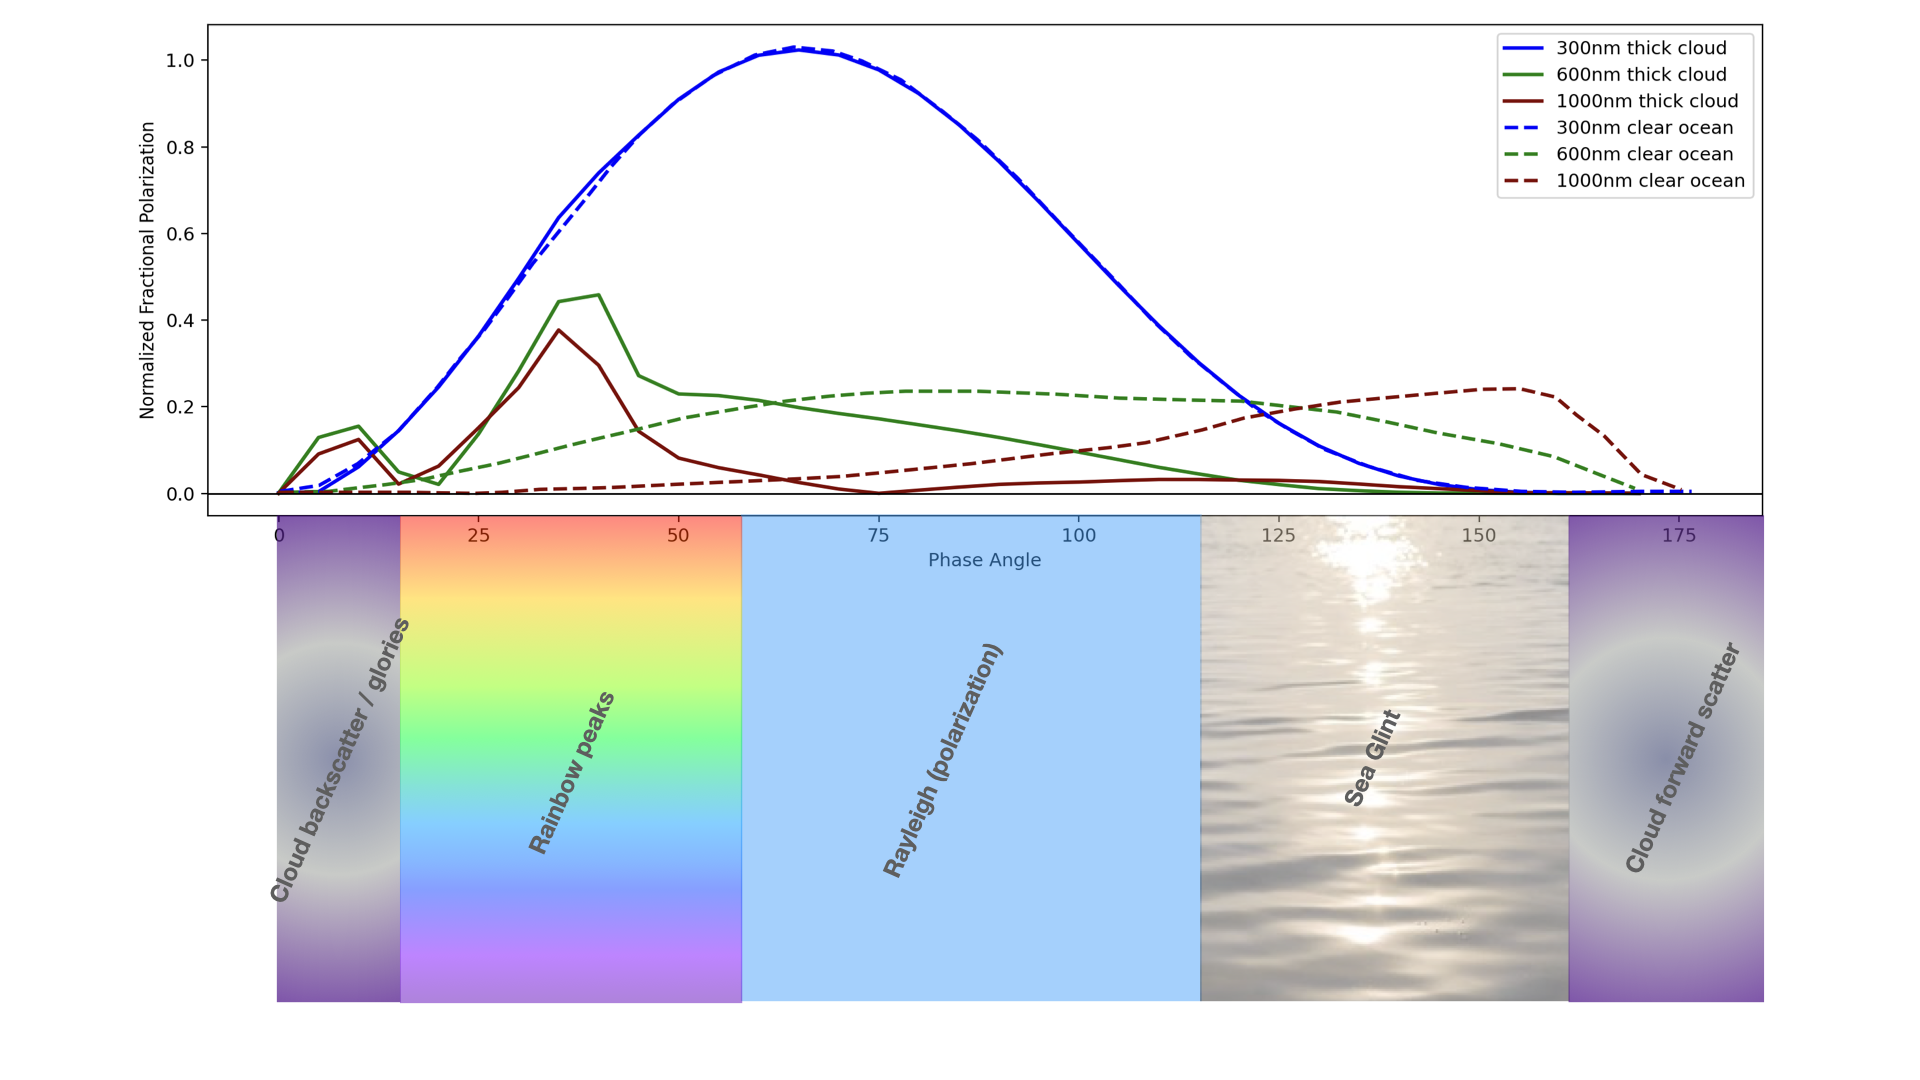
\includegraphics[width=\linewidth]{figures/Fig1IWAPol.png}
   \caption{BOTT PLOT this is a holder until Kim updates the figure}
    \label{fig:bottplot}
\end{figure*}

\textcolor{red}{introduce motivation, specs for habitable worlds observatory and the document we got the target list from.}

\textcolor{blue}{Habitable worlds bit}

The National Academy of Sciences Astronomy \& Astrophysics 2020 Decadal Survey \citep{decadal} recommended the first in a new \enquote{Great Observatories} program a telescope with the capability to detect signatures of habitability for about 25 habitable zone planets. This assertion requires an instrument with a coronograph capable of high contrast imaging in the optical-near infrared. Following this release, NASA recently announced the start of the development of the Habitable Worlds Observatory (HWO). The precursor technology recommended by the Decadal Survey also lists "direct imaging to probe polarized ocean glint on terrestrial planets" as one of the priority capabilities (\citet[Box E.1 in][]{decadal}) for ground and space-based observatories.
The performance and precise characteristics of this telescope (on-axis or off-axis, exact diameter, type of segmentation, type of coronagraph) are still to be determined. The development will be heavily influenced by the LUVOIR \citep{LUVOIR2019} and HabEx \citep{HabEx_2020} preparatory studies.  The Inner Working angle (\IWA) of the resulting telescope will be dependent on these choices, which in turn will have a significant impact on the expected exo-Earth yield \cite{Stark2019_exoplanetyield}.


Extreme Coronagraph for Living Planetary Systems (ECLIPS) coronograph for LUVOIR was a proposed \SIrange{200}{2000}{\nano\meter} instrument for exoplanet characterisation, with a similar coronagraph operating between \num{450} and \SI{1800}{\nano\meter} planned for HabEx. 
POLLUX, a proposed UV instrument for the LUVOIR study could also allow the detection of polarised light from hot Jupiters at \SI{300}{\nano\meter} \citep{Bouret2018_pollux}.  However, the challenges associated with the design of a coronagraph in UV are enormous, and it is unlikely that the HWO will include a UV high-contrast instrument sensitive to Earth-like planets.


%We ignore contrast in this study
%OWA -> should go in discussions

\textcolor{blue}{Science motivation below: Kim}\\
\textbf{Why Polarization curves worth looking at [Kim]}
%compare to features in nonpol (strength rainbow); current capabilties?

 Phase curves of planets are more complex than simple Lambertian curves. 
 The phase curve of an edge on system in unpolarized light is dominated by the reflectance and backscatter of the surface, clouds, and atmosphere. Though this behaviour is not Lambertian, the planet will, in general, get brighter at fuller phases (small scattering angles) with a peak at full phase from cloud backscatter \citet[see, for example,][]{kopparla2018}. In cases where surface liquid (sea) is present, the specular reflection can create a notable addition to the phase curve at broad scattering angles near crescent phase \citep{Robinson_2010}. Exoplanet phase curves can also contain a rainbow signature at gibbous phases (moderately narrow scattering angles), though this is a small feature in comparison to the reflectance.

 In polarized light, additional structure in the phase curve can enable phenomena like ocean glint, rainbows, and the Rayleigh scattering to be more easily distinguished.  Notably, in the polarized phase curve the rainbow may be an especially strong feature and the maximum reflectance signal (from Rayleigh scattering) occurs 

 


%Polarimetry provides the possibility to detect molecules, hazes, clouds and different surfaces  as they all produce unique polarization signatures which cannot be disentagled by using broadband flux alone. Polarimetry measurements of terrestrial exoplanet atmospheres therefore have the potential to provide empirical constraints on atmospheric properties that are inaccessible through other observational techniques. Polarimetry has previously played an important role in the understanding of solar system planet atmospheres, for instance, polarimetric measurements of Venus’ atmosphere suggested that the upper atmosphere of Venus is dominated by a haze of liquid sulphuric acid droplets \citep{Venus74}, which has been confirmed by in situ observations.

\textbf{Why rainbow worth it [Kim]} %calc; retrieve species including for non terrestrials; droplet liklihood of liquid surface; lit review bailey et below

%The rai

\textbf{Why glint [Kim]}
% probe of surface conditions; habitability

%\cite{2006astro.ph.10518M} first noted the potential for photometric and polarimetric scattered light phase to detect oceans on terrestrial exoplanets.   --> No it was talked about previous to this, per the paper cited here in fact... "Stam & Hovenier(2006) independently examined the observability of the polarized signatures of an Earth-likeextrasolar planet, including Rayleigh scattering and sea-surface glint. Schneider (2006) had similar ideas." -KB

%\cite{2008Icar..195..927W} simulated photometric and polarimetric phase curves of directly imaged terrestrial planets. They noted that surface oceans would be detectable because they are a) less reflective near full phase, 
% not following what you mean here -KB
%b) more reflective at crescent phases, and c) exhibit a peak in polarization at crescent phases. \cite{Zugger_2010} simulated photometric and polarized phase variations for planets including the effects of partial cloud coverage and ocean waves. Although the presence of clouds and atmospheric Rayleigh scattering weaken the signal of an underlying ocean, they again find that oceans are detectable and distinguishable from other sources of polarization. \cite{2010ApJ...721L..67R} compared observations of the Earth's scattering phase curve to simulations; they found .
%\citet{Zugger_2011} note that ocean glint might be observed in near infrared opacity windows, because of the reduced Rayleigh scattering at long wavelengths. This has the added advantage of minimizing the latitude--albedo effect, which could otherwise be a false-positive for photometric brightening at crescent phases due to glint \citep{2012ApJ...752L...3C}. \cite{2019A&A...626A.129T} simulated the photometric and polarimetric signatures of terrestrial planets with inhomogeneous clouds. \cite{2022A&A...664A.172T}


%cloud coverage paper in polarisation :
%\cite{rossi17} computed flux and polarisation of reflected starlight for different types of cloud cover on Earth-like planets and determined different types of cloud cover can be distinguished from each other. %Alternative options or papers here.... Kim can write this tomorrow , needs other Stam, Karalidi, Kopparla, maybe Gordon, need to reference rainbows in Bailey paper.  Look at citations in Gordon paper (our bib)... he has a really thorough lit review --KB

\textbf{In this paper we...}
% We minimally explore the contrast ratio as we are primarily exploring whether these scattering angles are reachable with inner working angle and outer working angle considered.

% We do not consider the particulars of specific planet scenarios as that work is completed by foward models

%We do not separate Stokes parameters as we are interested in where the net signal is achievable with IWA and OWA. 



%%%%%%%%%%%%%%%%%%%%%%%%%%%%%%%%%%%%%%%%%%%%%%%%%%%%%%%%%%%%%%%

%\section{Plots to Include}
%\label{sec:plots}
%\begin{enumerate}
%    \item \st{Cartoon defining various phase angles: orbital phase, scattering phase, $\beta$ ? (Sophia)}
%    \item Bott plot: annotated polarized and unpolarized phase curves for ocean world and cloudy worlds (Kim)
%    \item \st{3x3 cartoon showing effect of inclination and IWA compared to orbit (Sophia)}
%    \item Cumulative distribution functions, both simple (circular, edge-on), bit more realistic (circular, but range of inclinations), and full-on (range of inclinations and eccentricities). Max \& Matthew
%    \item Scatter plot of stellar effective temperature vs system distance (Timmy)
%\end{enumerate}
 



\section{Methods/simulations}
\subsection{HWO and Stellar Sample}
%\textcolor{blue}{Merge the 2 sections here into "Assumed technical specifications and sample"? I don't think this needs to be 2 subsections}
The HWO is still in the early stages of development, and the exact telescope and instrument design is undecided. 
In this work, we assume a \SI{6}{\meter} primary mirror, which is the currently favoured design for the observatory.

HWO will utilise a coronagraph to suppress the stellar light and facilitate high contrast observations of their faint exoplanet companions.  The IWA of the coronagraph is currently undecided and will be driven by both the science requirements and technological limitations. 
In this work, we investigate the scattering phase coverage obtainable for several choices for the IWA of the observatory. We also consider the Outer Working Angle (OWA) but for most targets this is not a limiting factor.

For ease of comparison, \cref{tab:IWA_OWA} indicates the angular separations corresponding to multiples of $\lambda / D$ for a \SI{6}{\meter} telescope at a wavelength of $\lambda = \SI{700}{\nano\meter}$.

\begin{table}
    \centering
    \caption{
        Conversion between $\lambda / D$ and mas for different wavelengths. \textbf{We should use consistent wavelengths for this table, for the Bott Plot, and for the M\&M cumulative distribution function. Also update to use the only wavelength we choose}
    }
    \label{tab:IWA_OWA}
    \begin{tabular}{ c c c c } 
    \toprule
     & $\lambda/D$ & mas (at \SI{600}{\nano\meter}) & mas (at \SI{700}{\nano\meter}) \\
    \midrule
    \midrule
    IWA & 1 & 21 & 24\\
    IWA & 2 & 42 & 48\\
    IWA & 3 & 63 & 72\\
    IWA & 4& 84& 96\\
    \midrule
    OWA & 32 & 660 & 770 \\
    OWA & 64 & 1320 & 1540\\
    \bottomrule
    \end{tabular}
\end{table}


%\subsection{Stellar sample and assumed planet parameters} 
We use the NASA Exoplanet Exploration Program's Mission Star List for the Habitable Worlds Observatory.%
\footnote{\url{https://exoplanets.nasa.gov/internal_resources/2645_NASA_ExEP_Target_List_HWO_Documentation_2023.pdf}}
This list comprises $\sim$160 stars, the majority of which are Sun-like dwarfs; 66~F~dwarfs, 55~G~dwarfs, 40~K~dwarfs, and 3~M~dwarfs.
The target list is constructed assuming a maximum planet magnitude of $R_c = 31$ and a contrast floor of \num{2.5e-11}. %with an occurrence rate of
%rocky planets in the optimistic habitable zone to be $\eta_{\oplus}$ = 0.24 \citep{decadal}. 
The corresponding adopted
habitable zone limits are a semi-major axis of \SIrange{0.95}{1.67}{\au} for a solar twin, planet sizes between \SIrange{0.8}{1.4}{} Earth radii, and for non-solar stars, scale as square root of the
bolometric luminosity normalized to the Sun. This range of orbital separations
corresponds to the \enquote{conservative habitable zone} \citep{kasting93, kopparapu13}.

The authors of the report determined that these are the nearby stars (maximum distance \SI{25}{\parsec}) for which exo-Earths would be the most observable for an imaging survey of habitable zones with a \SI{6}{\meter} telescope.



\subsection{Maximum scattering phase angle coverage}
\label{sec:Delta_phi}

The coronagraph, while necessary for observing faint exoplanets, can obscure part of the planet's orbit. 
As demonstrated in \cref{fig:orb-grid}, this can prevent the planet being detected at high and low scattering angles. 
In this section, we derive the minimum ($\phi_\mathrm{min}$) and maximum ($\phi_\mathrm{max}$) scattering phase angles accessible for a given orbit of semi-major $a$ (in \si{\au}), line of sight inclination $i$, star distance $d_*$ in parsecs (\si{\parsec}) and for a given inner working angle of the instrument \IWA (in milliarcseconds). 
We define the inclination $i$, such that $i=0$ corresponds to a face-on orbit. 

\begin{figure*}%[t]
   \centering
   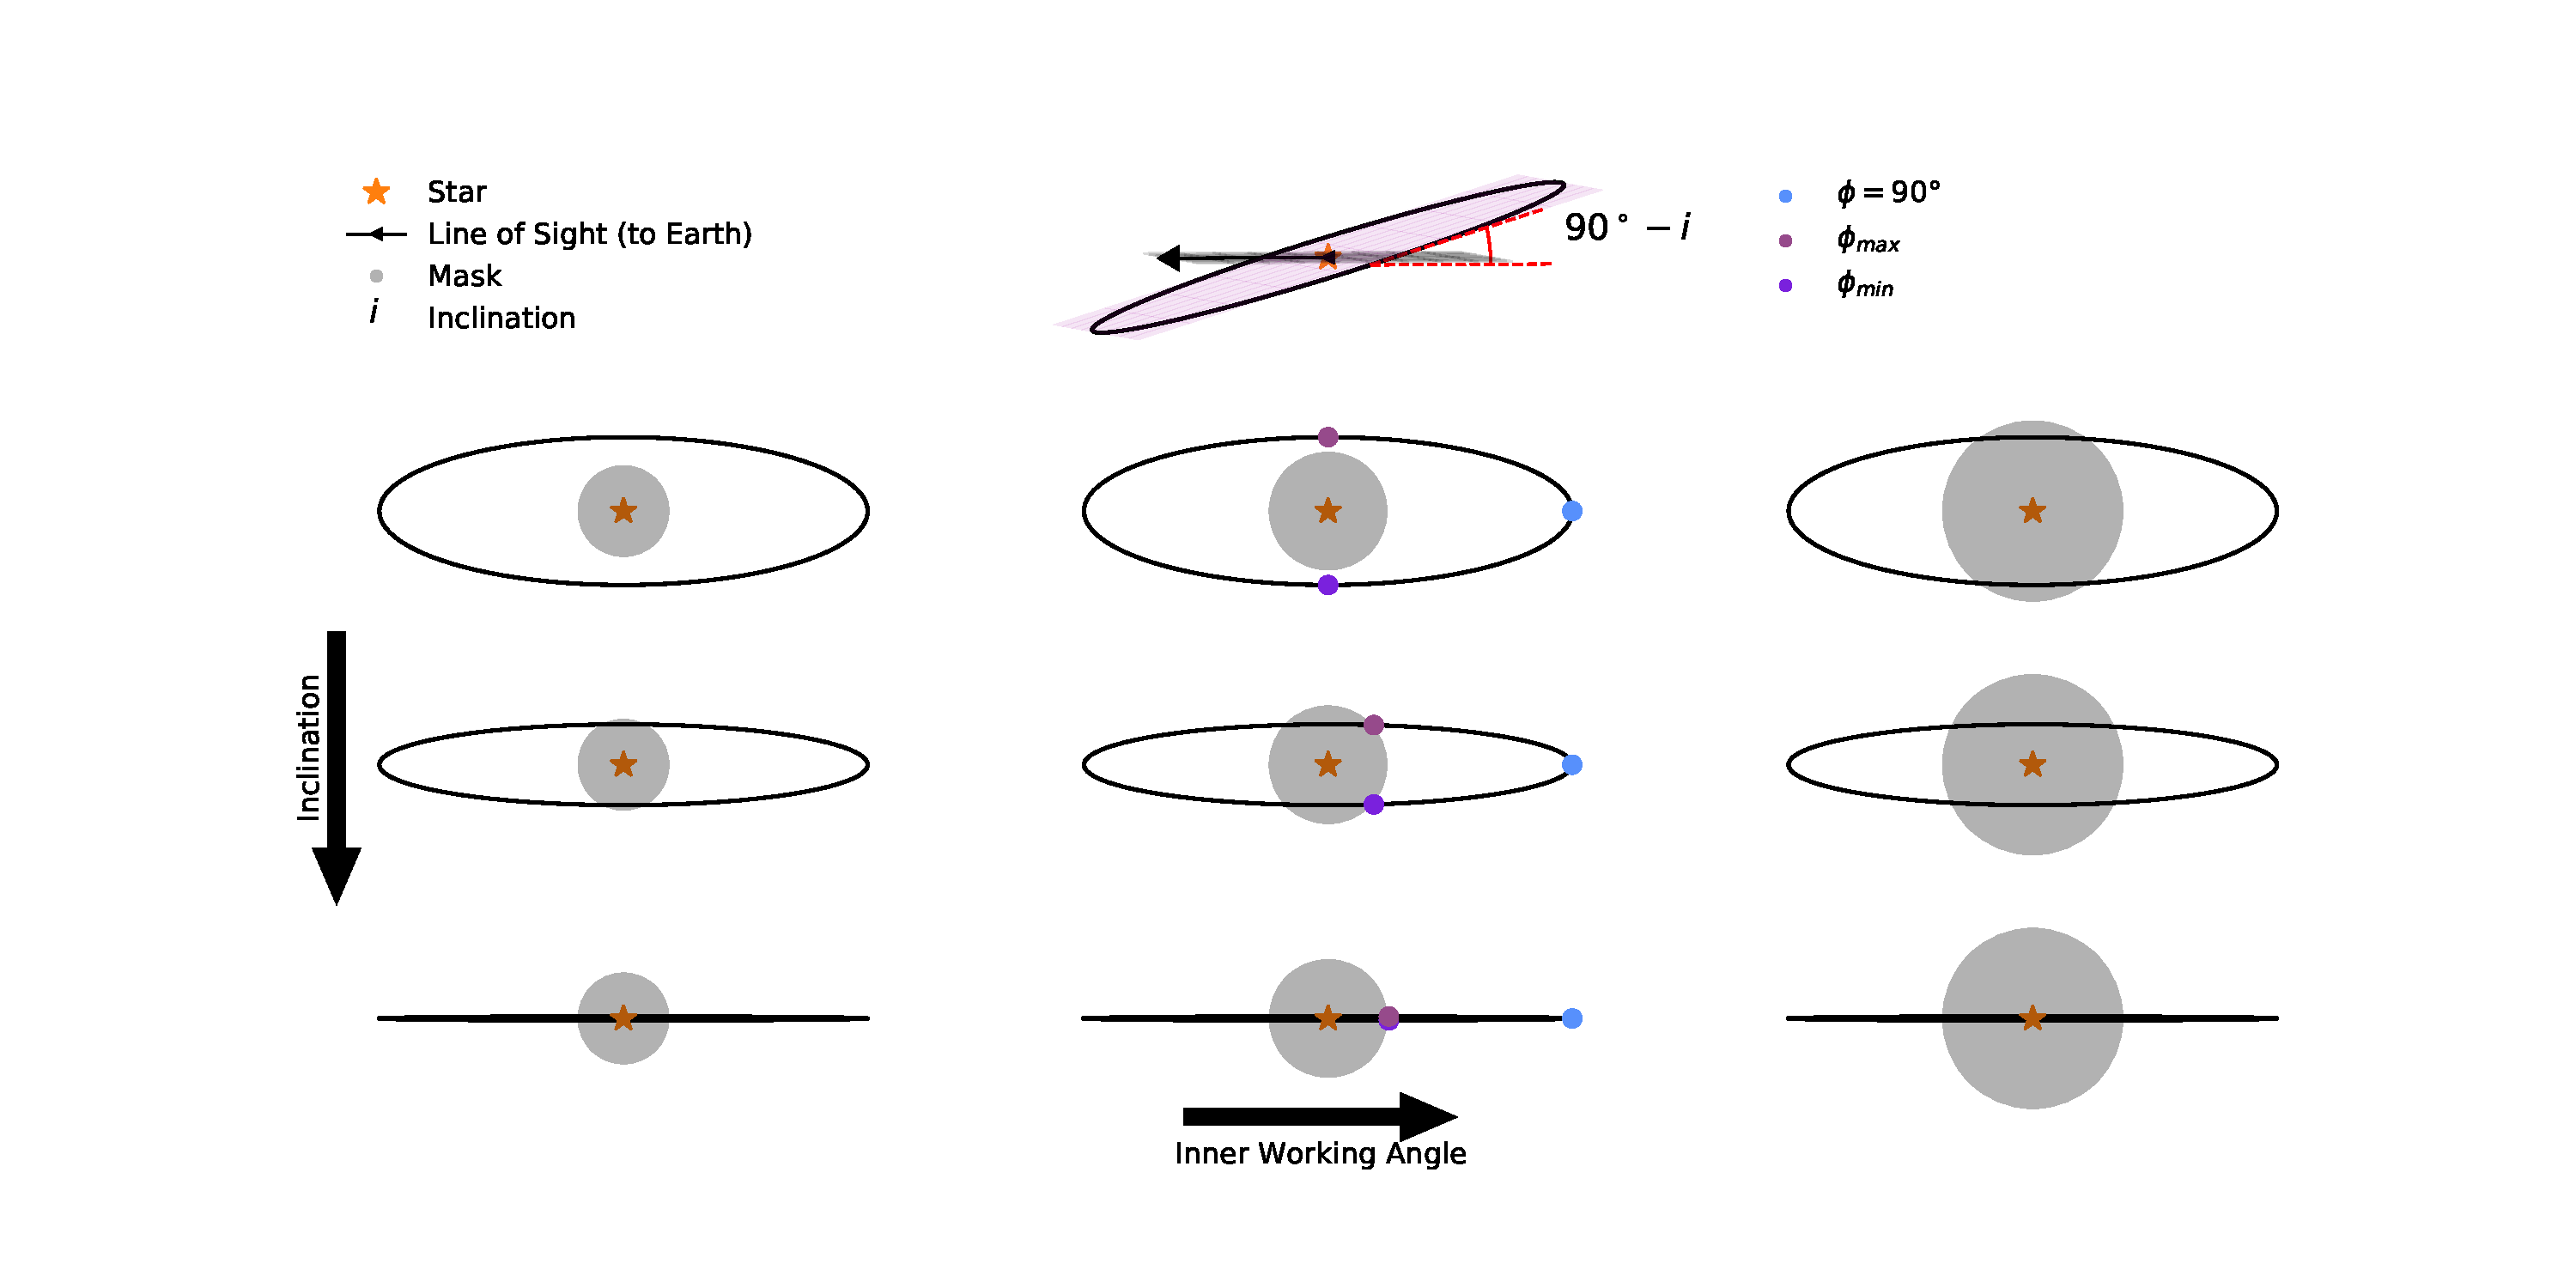
\includegraphics[width=0.99\textwidth]{figures/orb-grid.pdf}
   \caption{
        The scattering phase angles accessible to a direct imaging mission can be limited by orbital inclination or by the coronagraphic inner working angle. 
        If the orbital inclination is close to face-on (top panels) then the scattering phase angles probed throughout an orbit are limited by inclination; for circular orbits accessible scattering phases are $\phi \in 90^\circ \pm i$. 
        For orbital inclinations close to edge-on (bottom panels) the planet goes through all phases, but the scattering phase angles near 0$^\circ$ and 180$^\circ$ are not accessible due to obscuration by the coronagraph mask; for circular orbits, the accessible scattering phases are $\phi \in 90^\circ \pm \arcsin({\rm IWA}\cdot d_*/a)$.
    }
    \label{fig:orb-grid}
\end{figure*}

In the non-eccentric case (i.e., with a circular orbit and where the coronagraphic mask centred on the star), $\phi_\mathrm{min}$ and $\phi_\mathrm{max}$ are symmetric about 90 degrees (). 
We define the angle $\Delta \phi$ such that: 
\begin{equation}
    \label{eq:Delta_phi}
    \Delta \phi 
    = \phi_\mathrm{max} - \phi_\mathrm{min}
    =  2(\phi_\mathrm{max} - 90) 
    =  2(\phi_\mathrm{min} + 90)
\end{equation}


For a given system with inclination $i$, we have identified 2 regimes, shown in \cref{fig:orb-grid}:

(1)~If the inclination is face-on enough such that the coronagraph mask does not cover any part of the projected orbit on-sky, then the maximum scattering phase angle coverage depends solely on the disk inclination ;

(2)~When parts of the disk (minimum and maximum scattering phase angles) are hidden by the focal plane mask, the scattering phase angle coverage does not depend on the inclination and only on the IWA and orbit semi-major axis. In this section, we derive the analytical formula for this case in the circular orbit case. 

%\begin{figure}%[t]
%    \centering
    % 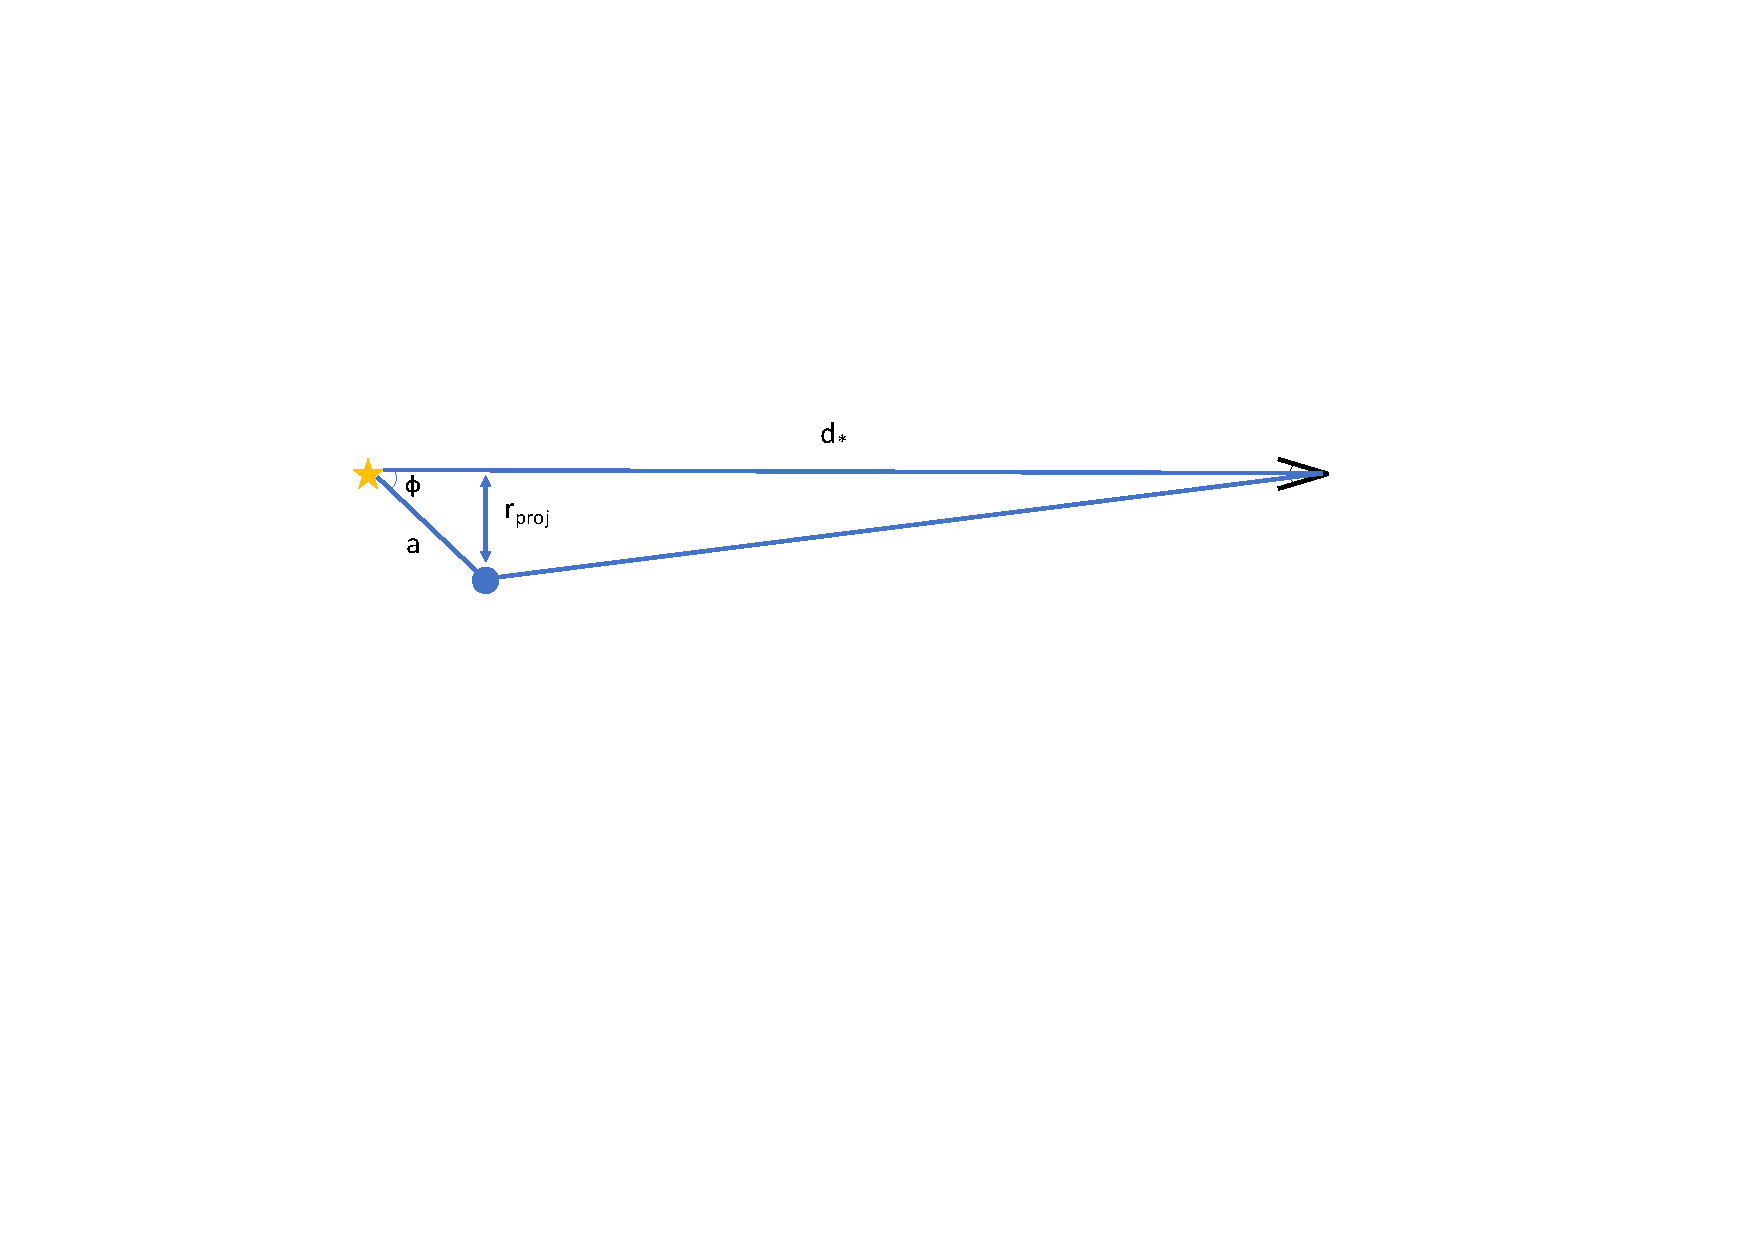
\includegraphics[width=\linewidth]{figures/scattering_angles.pdf}
%    \includestandalone{figures/scattering-phase-angle}
%    \caption{
%        The angular separation, $\varepsilon$, of a planet orbiting with semi-major-axis $a$ about a star a distance $d_*$ from the observer. 
%        The scattering phase angle is $\varphi$. 
%        The smallest accessible scattering phase angle occurs when the angular separation equals the coronagraph inner working angle: $\varphi_{\rm min} = {\rm IWA} \cdot d_*/a$.
%    }
%    \label{fig:scattering_angles}
%\end{figure}

%From \cref{fig:scattering_angles}, we deduce that for all points on the orbit, the scattering angle $\varphi$ satisfies:
\begin{equation}
    \sin(\varphi) = \frac{r_\mathrm{proj}}{a}
\end{equation}
with $r_\mathrm{proj}$ the on-sky projected planet distance (in \si{\au}), $a$ the distance to the star (constant in this section, in \si{\au}). 

$\varepsilon$ is the angular separation of the planet at a given point of the orbit ($r_\mathrm{proj} = \delta d_*$). 
We access the minimum scattering angle when the projected distance reaches the inner working angle separation $\delta = \mathrm{IWA}$. 
Using \cref{eq:Delta_phi}, we deduce:

\begin{equation}
    \cos\left(\dfrac{\Delta \phi}{2}\right) = \frac{\mathrm{IWA \cdot d_*}}{a}
\end{equation}

We now deduce the 2 regime equation for all cases (circular orbit): 
\begin{equation}
\label{eq:Delta_phi_max}
    \Delta \phi = 
    \begin{cases}
        2 \cdot i & \textrm{for} \cos(i) > \dfrac{\mathrm{IWA}\cdot d_* }{a}
  \\ 
        2 \cdot \cos^{-1}\left(\dfrac{\mathrm{IWA}\cdot d_* }{a}\right)  & \textrm{for} \cos(i) < \dfrac{\mathrm{IWA}\cdot d_* }{a}
    \end{cases}\,.
\end{equation}

\subsection{Edge-on circular orbits}
\label{sec:edge-on}
We initially performed a simple test considering only edge-on circular orbits. This gives an upper limit for circular orbits for the visible scattering phase range as a function of inclination. Fig. \ref{fig:scatterplot} shows $\Delta \phi$ for the systems in the target list assuming a $3 \lambda / D$, at $\SI{600}{\nano\meter}$, coronograph. This optimistic case indicates that it will be possible to observe Rayleigh scattering for all targets and that rainbows will be accessible in some cases.

\begin{figure*}
    \centering
    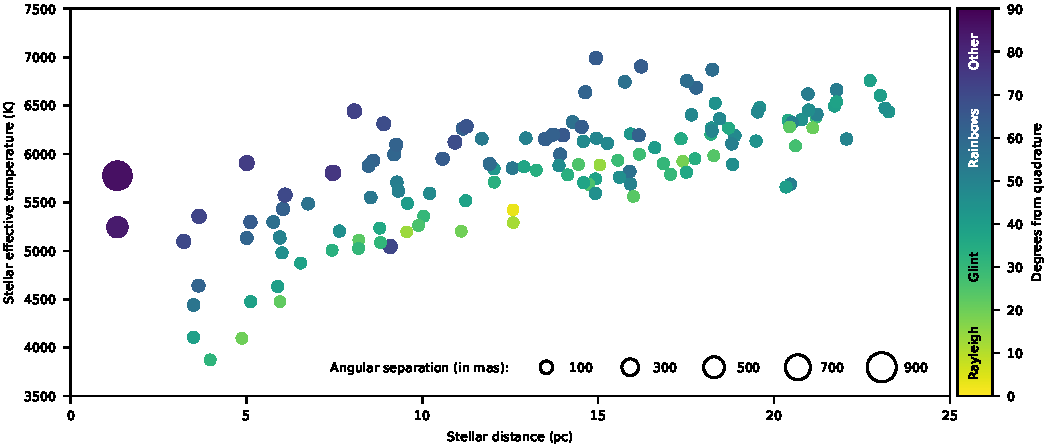
\includegraphics{figures/scatterplot.pdf}
    \caption{
        Scatter plot at 3 $\lambda/D$ for the target sample showing stellar effective temperature and stellar distance. 
        The size of the points represents the angular separation of the star and planet in milliarcseconds as presented in the target list. The colour of the points shows the atmospheric phenomenon that can be detected with darker colors including all lighter (yellow) color phenomenon. Thus dark blue points are systems which have the most key features, as systems in which the angles required to see the rainbow are probed will also have the angles required to see the Rayleigh scattering probed.
    }
    \label{fig:scatterplot}
    \script{create-scatterplot.py}
\end{figure*}

\subsection{Assumed planet parameters}

As shown in \cref{sec:Delta_phi}, $\Delta \phi$ depends on the angular separation, inclination and eccentricity of the planets orbit. 
We use the angular separation for an Earth-Like planet with the same instellation as Earth which is provided in the input star list. 
The inclination $i$ is sampled such that $\cos(i)$ follows a uniform distribution, $\cos(i) \sim \mathcal{U}(0, 1)$.

\subsection{Making Contrast Curves}
\textbf{Kim and David}
%

% \subsection{Monte Carlo Simulations}
% \label{sec:montecarlo}
% For each star on the HabWorlds target list, we generate XX hypothetical habitable planets at the Earth-equivalent-flux semi-major axis.
The reflected flux and polarisation are not constant as a function of scattering phase angle. This is due to a combination of the changing illumination fraction of the exoplanets Earth facing surface and scattering effects. These are modelled using ...

\section{Results}

\subsection{Circular randomly inclined orbits}
\label{sec:circular}
For each star on the HabWorlds target list, we generate XX hypothetical habitable planets at the Earth-equivalent-flux semi-major axis. The orbital inclinations are randomly drawn from a distribution uniform in $\cos i$. We then use Eqn \ref{eq:Delta_phi_max} to determine the range of accessible scattering phase angles for each hypothetical planet. Figure blah shows the cumulative distribution for the most extreme scattering phase angles accessible for the HabWorlds target list, depending on the choice of inner working angle.  

\textbf{Is there a plot for this?}

\subsection{Eccentric randomly inclined orbits}
\label{sec:eccentric}
We repeat the Monte Carlo simulation from section \ref{sec:circular} assuming the orbital eccentricity follows a beta distribution with shape parameters $a=0.867$ and $b=3.03$ (cf. \citet{Guimond_2019} and references therein). We randomly drew 1000 eccentricities from the beta distribution for each star and determined the orbits. We then filtered on $\IWA$ for multiples of 1, 2, 3 and 4 $\lambda / D$, before identifying which targets would be observable at the scattering phase angles where ocean glint, rainbows or the Rayleigh peak occur. Figure \ref{fig:ball-o-yarn} shows a sample of the generated orbits with the filtered \IWA's. Each plot has been scaled such that the habitable zone occupies the same radius hence the \IWA's vary in apparent size compared to the orbit. 

\begin{figure*}
    \centering
    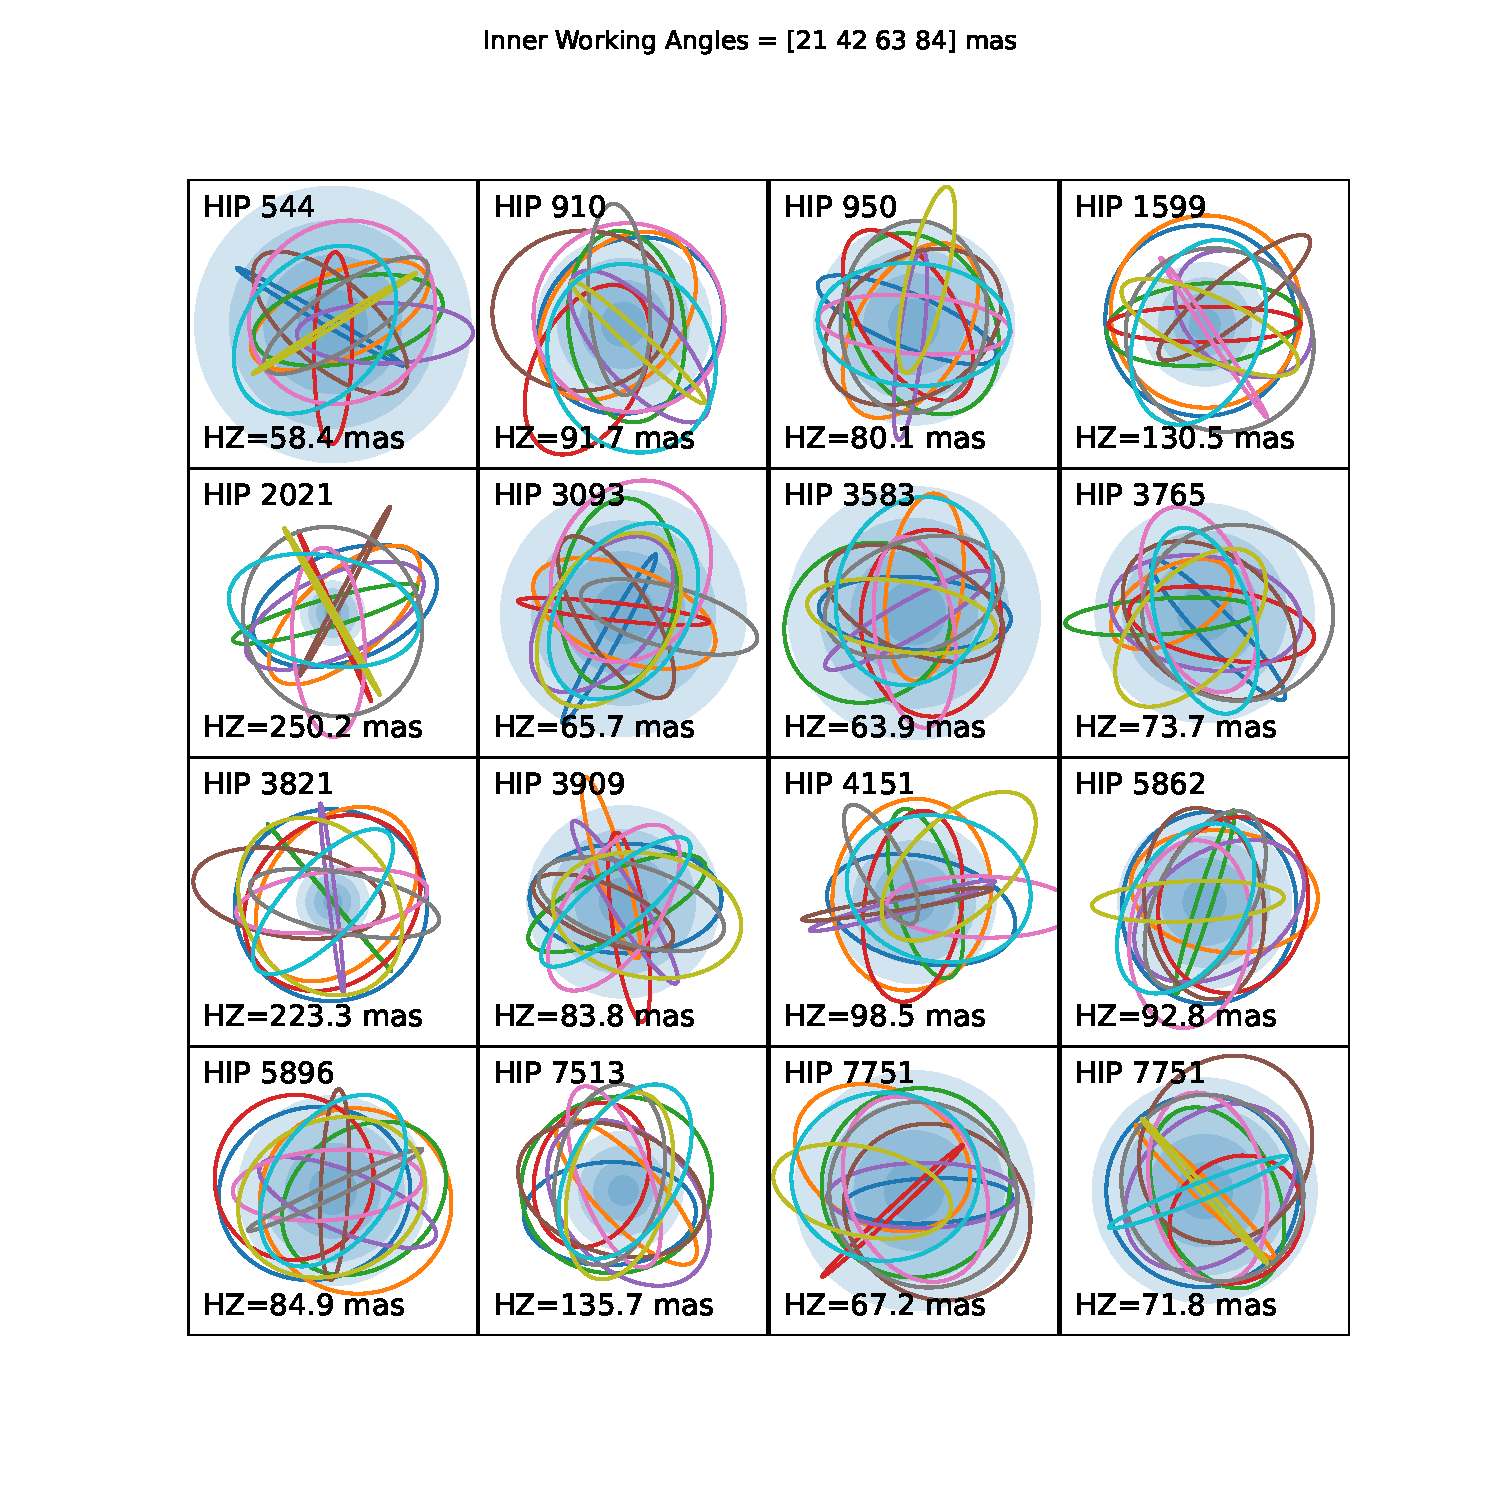
\includegraphics[width=\textwidth]{figures/madness.pdf}  
    \caption{
        A example of the eccentric orbits generated for the stellar sample. The orbits are scaled by the Earth-equivalent flux distance. The shaded region indicates \IWA's of 1, 2, 3 and 4~$\lambda / D$ corresponding to 21, 42, 63 and 84 mas. The \IWA can significantly affect the range of scattering phases observable with each orbit.
    }
    \label{fig:ball-o-yarn}
\end{figure*}


 
\begin{figure*}
    \centering
    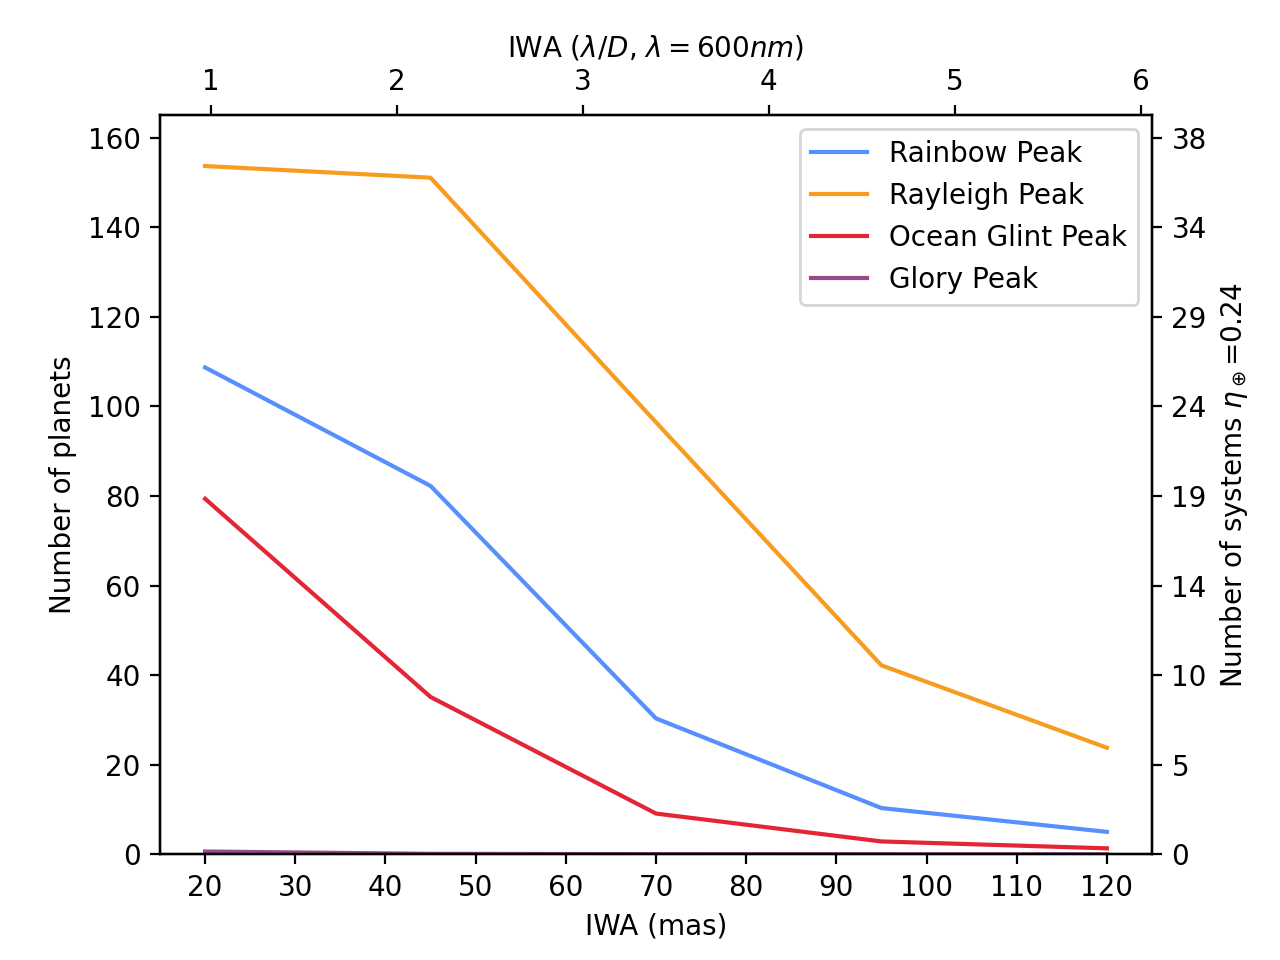
\includegraphics[width=0.6\textwidth]{figures/features_plot_peak.png}  
    \caption{
        Number of systems vs inner working angle
    }
    \label{fig:accessible_phase_angles}
\end{figure*}

\subsection{The glory of Alpha Cen}
\label{sec:ealpha-cen}
\textbf{Glory science, what it tells us (Kim)}
% Kim will write para on science of glory (what tells us, vaguely why appears here)

\subsection{Contrast Curves}
\label{sec:contrast}

\section{Discussion}
What did we determine? Can we actually detect this stuff for anything in this sample? Do we need to not something about things like A stars which are not included in the sample - they were rejected by the list creators - do we need to comment on this? 



\section*{Software Data Availability}
%Maybe we could upload the code that we used for our analysis / plots somewhere?
%Just for full transparency / reproducibility?
The NASA ExEP target list containing the data used for these simulations is available online.% 
\footnote{\url{https://exoplanets.nasa.gov/exep/science-overview/}}
This work has made use of \textsf{numpy}
 \citep{NumPy2020}, \textsf{scipy} \citep{scipy_2020}, \textsf{matplotlib} \citep{matplotlib2007}, and \textsf{astropy},\footnote{\url{https://www.astropy.org}} a community-developed core Python package and an ecosystem of tools and resources for astronomy \citep{astropy:2013, astropy:2018, astropy:2022}.




\section*{Acknowledgements}
The workshop on which this manuscript is based was made possible thanks to the logistical and financial support of the Lorentz Center, Leiden, Netherlands. This workshop was supported by NOVA  and by the European Research Council (ERC) under the European Union's Horizon 2020 research and innovation programme (grant agreement n°866001 - EXACT).

This research has made use of NASA's Astrophysics Data System Bibliographic Services and the SIMBAD database, operated at CDS, Strasbourg, France. 

SRV acknowledges funding from the European Research Council (ERC) under the European Union’s Horizon 2020 research and innovation program under grant agreement No 805445.
SLC acknowledges support from an STFC Ernest Rutherford Fellowship. 
TDG acknowledges funding from the Max Planck ETH Center for Learning Systems.
Specific grant funding and any other specific requirements
KMB acknowledges support from NASA Habitable
Worlds grant No. 80NSSC20K152, and previous support for related work supported by NASA Astrobiology Institute's Virtual Planetary Laboratory under Cooperative Agreement Number NNA13AA93A.

% Add references
\bibliographystyle{mnras}
\bibliography{bib}

\end{document} 